%%%%%%%%%%%%%%%%%%%%%%%%%%%%%%%%%%%%%%%%%%%%%%%%%%%%%%%%%%%%%%%%%%%%%%%%%%%%%%%%%%%%
%Do not alter this block of commands.  If you're proficient at LaTeX, you may include additional packages, create macros, etc. immediately below this block of commands, but make sure to NOT alter the header, margin, and comment settings here. 
\documentclass[12pt]{article}
 \usepackage[margin=1in]{geometry} 
\usepackage{amsmath,amsthm,amssymb,amsfonts, enumitem, fancyhdr, color, hyperref,comment, graphicx, environ,mathtools, bbm, tikz, setspace, cleveref,listings, dcolumn}
\usepackage{array, multirow, caption, booktabs}
\usepackage{lscape}
\usepackage{ mathrsfs }
\usetikzlibrary{matrix,positioning}
\tikzset{bullet/.style={circle,draw=black,inner sep=8pt}}
\DeclareMathOperator*{\argmax}{arg\,max}
\DeclareMathOperator*{\argmin}{arg\,min}
\DeclareMathOperator*{\Var}{\text{Var}}
\DeclareMathOperator*{\Cov}{\text{Cov}}

\DeclarePairedDelimiter\norm{\lVert}{\rVert}%
\newtheorem{theorem}{Theorem}
\newtheorem{lemma}[theorem]{Lemma}
\DeclareMathOperator{\eps}{\varepsilon}
\doublespacing
\DeclarePairedDelimiter\abs{\lvert}{\rvert}%
\pagestyle{fancy}
\setlength{\headheight}{65pt}
\newenvironment{problem}[2][Problem]{\begin{trivlist}
\item[\hskip \labelsep {\bfseries #1}\hskip \labelsep {\bfseries #2.}]}{\end{trivlist}}
\newenvironment{sol}
    {\emph{Solution:}
    }
    {
    \qed
    }


%%%%%%%%%%%%%%%%%%%%%%%%%%%%%%%%%%%%%%%%%%%%%%%%%%%%%%%%%%%%%%%%%%%%%%%%%%%%%%%%%


\usepackage{xcolor}
 
 


%%%%%%%%%%%%%%%%%%%%%%%%%%%%%%%%%%%%%%%%%%%%%

\rhead{Asha Bharadwaj, Caitlin Dutta, John Higgins, Alexis Smith\\Econ 899 \\ 20 December, 2022} 

%%%%%%%%%%%%%%%%%%%%%%%%%%%%%%%%%%%%%%%%%%%%


%%%%%%%%%%%%%%%%%%%%%%%%%%%%%%%%%%%%%%

\begin{document}

\begin{problem}{1}
\end{problem}
\begin{sol}
    The state space is the Cartesian product $\{0, 5, \ldots, 45\} \times \{0, 5, \ldots, 45\}$.
\end{sol}
\begin{problem}{2}
\end{problem}
\begin{sol}
    We calculated the payoffs in the static game and plotted the payoffs for firm 1 (without loss of generality, since they are symmetric):
    \begin{center}
        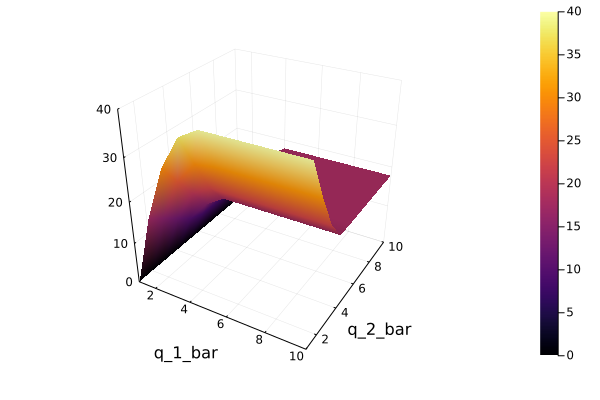
\includegraphics[scale=0.5]{piplot.png}
    \end{center}
\end{sol}
\begin{problem}{3}
\end{problem}
\begin{sol}
The Markov Perfect Equilibrium is characterized by the following two conditions:
\begin{align}
    x_i(\omega) = R_i(x_j(\omega)\mid \omega) \quad \text{for all } i,j = 1,2\\
    V_i^x(\omega) = \pi_i(\omega) - x_i(\omega) + \beta \sum_{\bar{q}_i'} W_i^x(\bar{q}_i'\mid \omega) P(\bar{q}_i' \mid \bar{q}_i, x_i) \quad \text{for all} i,j = 1,2
\end{align}
where $R_i(\cdot \mid \omega)$ is $i$'s best response function, $\pi_i(\cdot)$ is the payoffs of the static game, $W_i^x(\bar{q}_i) = \sum_{\bar{q}_2'} V_i^x(\bar{q}_i, \bar{q}_j') P(\bar{q}_j' \mid \bar{q}_j, x_j)$ represents the continuation value. 
\end{sol}
\begin{problem}{4}
\end{problem}
\begin{sol}
    We have plotted the strategy surface below:
    \begin{center}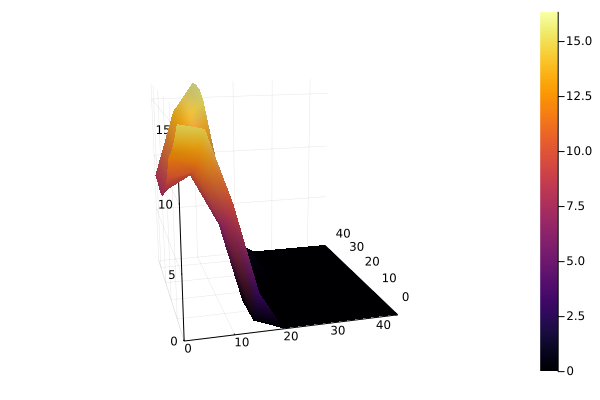
\includegraphics[scale=0.5]{xplot.png}\end{center}
    We also used the investment policy function to compute the transition matrix $Q(\omega'\mid \omega)$.
\end{sol}
\begin{problem}{5}
\end{problem}
\begin{sol}
    Starting at $\omega = (0,0)$ and simulating the evolution of the industry over 25 years 1,000 times, we obtain the following distribution over states $(\bar{q}_{1, 25}, \bar{q}_{2,25})$:
    \begin{center}
        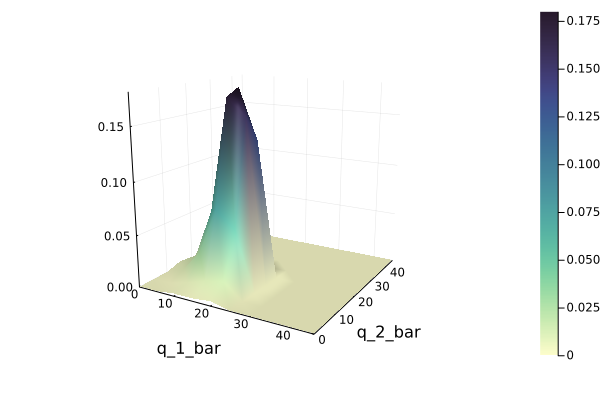
\includegraphics[scale=0.5]{simplot.png}
    \end{center}
\end{sol}

\end{document}